%https://tex.stackexchange.com/questions/164991/pgfplots-how-to-fill-bounded-area-under-a-curve-using-addplot-and-fill

%https://tex.stackexchange.com/questions/140312/tikz-shading-region-bounded-by-several-curves
%tikz para graficar areas

%http://latexcolor.com/

%https://www.tablesgenerator.com/
\PassOptionsToPackage{force}{filehook}

\documentclass{beamer}


\usepackage[utf8]{inputenc}
\usepackage{amsmath}
\usepackage{amssymb}% http://ctan.org/pkg/amssymb
\usepackage{amsfonts}
\usepackage{pifont}% http://ctan.org/pkg/pifont
%https://tex.stackexchange.com/questions/42619/x-mark-to-match-checkmark
\newcommand{\cmark}{\ding{51}}
\newcommand{\xmark}{\ding{55}}
%\usepackage{amsfonts}
\usepackage{graphicx} 
\usepackage{subcaption}
\usepackage{hyperref}
\usepackage{cancel}
\usepackage{wrapfig}
\usepackage{enumitem}
\usepackage{comment}
\hypersetup{
	colorlinks=true,
	linkcolor=blue,
	filecolor=magenta,      
	urlcolor=cyan,
}
\newtheorem*{proposicion}{Proposici\'on}
\newtheorem*{teorema}{Teorema}
\renewcommand*{\proofname}{Demostraci\'on}
\newtheorem*{ejercicio}{Ejercicio}
\usepackage{pgf,tikz}
\usetikzlibrary{positioning}
\usetikzlibrary{arrows,patterns}
\usetikzlibrary{arrows.meta}
\usepackage[spanish, activeacute]{babel} %Definir idioma español
\usepackage[utf8]{inputenc} %Codificacion utf-8
\usepackage{multirow}

%   Esconder las soluciones
\newif\ifhideproofs
\hideproofstrue %uncomment to hide proofs

\ifhideproofs
\usepackage{environ}
\NewEnviron{hide}{}
\let\solucion\hide
\let\endsolucion\endhide
\fi

\usepackage{color}
\usepackage{mathpazo}
\usepackage{hyperref}
\usepackage{multimedia}
\usepackage{graphicx}
\usepackage{textcomp}
\usepackage[spanish, activeacute]{babel} 
\usepackage{graphicx} 
\usepackage{booktabs}
\usepackage{cite}
\usepackage{hyperref}
\usepackage{multicol}
\usepackage{multirow,array}

\usepackage{mathrsfs}
%\usepackage{amssymb}

\usepackage{tabularx}
    \newcolumntype{L}{>{\raggedright\arraybackslash}X}
        %\newcolumntype{b}{>{\hsize=1.5\hsize}X}
    %\newcolumntype{s}{>{\hsize=.9\hsize}X}

\usepackage{amsthm}
\newtheorem{thm}{Teorema}
\newtheorem{lem}[thm]{Lema}
\newtheorem{axiom}[thm]{Axioma}
\newtheorem{prop}[thm]{Proposici\'on}
\newtheorem{coro}[thm]{Corolario}
\theoremstyle{definition}
\newtheorem{defn}{Definici\'on}
\DeclareGraphicsExtensions{.pdf,.jpeg,.png,.eps}
\usetheme{CambridgeUS}
\setbeamertemplate{navigation symbols}{}

%Paréntisis y otros
\newcommand{\cmc}{\overset{m.c.}{\rightarrow}}
\newcommand{\p}[1]{\left(#1\right)}
\newcommand{\cor}[1]{\left[#1\right]}
\newcommand{\lla}[1]{\left\{#1\right\}}
\newcommand{\eps}{\varepsilon}
\newcommand{\lol}{\mathcal{L}}
\newcommand{\RR}{\mathbb{R}}
\newcommand{\QQ}{\mathbb{Q}}
\newcommand{\NN}{\mathbb{N}}
\newcommand{\paren}[1]{\left(#1\right)}
\newcommand{\corc}[1]{\left[#1\right]}
\newcommand{\llav}[1]{\left\lbrace#1\right\rbrace}
\newcommand{\partt}[1]{\left(\text{#1}\right)}
\newcommand{\corctt}[1]{\left[\text{#1}\right]}
\newcommand{\llavtt}[1]{\left\lbrace\text{#1}\right\rbrace}
\makeatletter
\def\munderbar#1{\underline{\sbox\tw@{$#1$}\dp\tw@\z@\box\tw@}}
\makeatother

%\usepackage[scr=rsfs,cal=boondox]{mathalfa}
\usepackage[scr=esstix,cal=boondox]{mathalfa}

% \usepackage{mdframed}
% \newmdtheoremenv{solucion}{Soluci\'on}

% Enmarcar las soluciones
% \newenvironment{solu}
% {%
% \begin{framed}
%   \begin{solucion}
%   }%
%     {%     
%   \end{solucion}
% \end{framed}
% }

%   Esconder las soluciones
\newif\ifhideproofs
%\hideproofstrue %uncomment to hide proofs

\ifhideproofs
\usepackage{environ}
\NewEnviron{hide}{}
\let\solucion\hide
\let\endsolucion\endhide
\fi



%Graficos y cosas
\usepackage{amssymb}
\usepackage{tikz}
\usepackage{pgfplots}
\usepackage{mathtools}
\usepackage{xcolor}
%\pgfplotsset{compat=1.9}
\usepgfplotslibrary{fillbetween,decorations.softclip}
\pgfplotsset{compat = newest}
\usepackage{pst-func}
\usepackage{pstricks}
\usepackage{pst-plot}

% Comando para usar multiples footnotes en un align environment

\makeatletter
\newcommand{\AlignFootnote}[1]{%
    \ifmeasuring@
    \else
        \footnote{#1}%
    \fi
}
\makeatother

%https://tex.stackexchange.com/questions/82782/footnote-in-align-environment


\DeclareGraphicsExtensions{.pdf,.jpeg,.png,.eps}
%\usepackage{tikz}
%\usepackage{tikz-cd}
\usetikzlibrary{decorations}
%\usetikzlibrary{snakes}
%\usetikzlibrary{cd}

\useoutertheme{split}
\useinnertheme{rounded}


%\beamertemplatenavigationsymbolsempty  %removes navigation bar
\definecolor{rosee}{rgb}{0.7,0.05,0.25}
\definecolor{pacificorange}{cmyk}{0,.6,1,0} %approved Pacific colors 2010
\definecolor{pacificgray}{cmyk}{0,.15,.35,.60}
\definecolor{pacificlgray}{cmyk}{0,0,.2,.4}
\definecolor{pacificcream}{cmyk}{.05,.05,.15,0}
\definecolor{deepyellow}{cmyk}{0,.17,.80,0}
\definecolor{lightblue}{cmyk}{.49,.01,0,0}
\definecolor{lightbrown}{cmyk}{.09,.15,.34,0}
\definecolor{deepviolet}{cmyk}{.79,1,0,.15}
\definecolor{deeporange}{cmyk}{0,.59,1,18}
\definecolor{dustyred}{cmyk}{0,.7,.45,.4}
\definecolor{grassgreen}{RGB}{92,135,39}
\definecolor{pacificblue}{RGB}{59,110,143}
\definecolor{pacificgreen}{cmyk}{.15,0,.45,.30}
\definecolor{deepblue}{cmyk}{1,.57,0,2}
\definecolor{turquoise}{cmyk}{.43,0,.24,0}
\definecolor{gren}{rgb}{0.2,0.8,0.5}
\definecolor{orang}{rgb}{1,0.64,0}
\definecolor{amethyst}{rgb}{0.6, 0.4, 0.8}
\definecolor{dodgerblue}{rgb}{0.12, 0.56, 1.0}
\definecolor{fandango}{rgb}{0.71, 0.2, 0.54}
\definecolor{forestgreen(traditional)}{rgb}{0.0, 0.27, 0.13}
\definecolor{iris}{rgb}{0.35, 0.31, 0.81}
\definecolor{jazzberryjam}{rgb}{0.65, 0.04, 0.37}
\definecolor{mediumjunglegreen}{rgb}{0.11, 0.21, 0.18}
\definecolor{mediumpersianblue}{rgb}{0.0, 0.4, 0.65}
\definecolor{midnightgreen}{rgb}{0.0, 0.29, 0.33}
\definecolor{orangee}{rgb}{1.0, 0.5, 0.0}
\decimalpoint
% There are many different themes available for Beamer. A comprehensive
% list with examples is given here:
% http://deic.uab.es/~iblanes/beamer_gallery/index_by_theme.html
% You can uncomment the themes below if you would like to use a different
% one:
%\usetheme{AnnArbor} %boca
%\usetheme{Antibes} %azul y gris
%\usetheme{Bergen} %barra who where
%\usetheme{Berkeley} %bordes
%usetheme{Berlin} %blanco y azul
%\usetheme{Boadilla}
%\usetheme{boxes}
\usetheme{CambridgeUS}
%\usetheme{Copenhagen}
%\usetheme{Darmstadt}
%\usetheme{default}
%\usetheme{Frankfurt}
%\usetheme{Goettingen}
%\usetheme{Hannover}
%\usetheme{Luebeck}
%\usetheme{Malmoe}
%\usetheme{Marburg}
%\usetheme{Montpellier}
%\usetheme{PaloAlto}
%\usetheme{Pittsburgh}
%\usetheme{Rochester}
%\usetheme{Singapore}
%\usetheme{Szeged}
%\usetheme{Warsaw}

%\usecolortheme{beaver}
%\usecolortheme{whale}
%\usecolortheme{orchid}
%\usecolortheme{wolverine}
%\usecolortheme[named=pacificblue]{structure} %replaces the blue of Copenhagen with Pacific orange

\definecolor{myNewColorA}{rgb}{0,0,100}
\definecolor{myNewColorB}{rgb}{0,100,100}
\definecolor{myNewColorC}{rgb}{0,200,100}
\definecolor{myNewColorD}{rgb}{0,100,200}

%\setbeamercolor*{palette primary}{bg=myNewColorA, fg = black}
%\setbeamercolor*{palette secondary}{bg=myNewColorB, fg = black}
%\setbeamercolor*{palette tertiary}{bg=myNewColorC, fg = black}
%\setbeamercolor*{palette quaternary}{bg=myNewColorD, fg = black}

\setbeamercolor*{palette primary}{bg=rosee, fg = white}
\setbeamercolor*{palette secondary}{bg=gren, fg = white}
\setbeamercolor*{palette tertiary}{bg=-red!75!, fg = white}
\setbeamercolor*{palette quaternary}{bg=-red!75!, fg = white}



%\expandafter\def\expandafter\insertshorttitle\expandafter{%
 % \insertshorttitle\hfill%
  %\insertframenumber\,/\,\inserttotalframenumber}

%\mode
%<all>

%Para agrandar el espacio entre renglones de las tablas
%https://tex.stackexchange.com/questions/26690/how-to-add-extra-spaces-between-rows-in-tabular-environment
\renewcommand{\arraystretch}{2}

\usepackage{color, xcolor}
\definecolor{codegreen}{rgb}{0,0.6,0}
\definecolor{codegray}{rgb}{0.5,0.5,0.5}
\definecolor{codepurple}{rgb}{0.58,0,0.82}
\definecolor{backcolour}{rgb}{0.95,0.95,0.92}

\usepackage{listings}
\lstdefinestyle{mystyle}{
  backgroundcolor=\color{backcolour},   
  commentstyle=\color{codegreen},
  language = R,
  % commentchar=\#,
  keywordstyle=\color{magenta},
  numberstyle=\tiny\color{codegray},
  stringstyle=\color{codepurple},
  basicstyle=\ttfamily\footnotesize,
  breakatwhitespace=false,         
  breaklines=false,                 
  captionpos=b,                    
  frame=single,
  keepspaces=false,
  % numbers=left,                    
  % numbersep=pt,                  
  % columns=flexible,
  stepnumber=1,
  resetmargins=true,
  showspaces=false,                
  showstringspaces=false,
  showtabs=false,                  
  tabsize=1
}
\lstset{style=mystyle}
  

\def\mydate{\leavevmode\hbox{\twodigits\day/\twodigits\month/\the\year}}
\def\twodigits#1{\ifnum#1<10 0\fi\the#1}

\usepackage[final]{pdfpages}

% PARA AGREGAR IMAGEN EN EL FONDO DE LAS SLIDES
\usebackgroundtemplate%
%{%
 %
\includegraphics[width=\paperwidth,height=\pape%rheight]{slides1/fondo.png}%  
%}


\title{\color{black}{Análisis Estadístico}}
\subtitle{\color{rosee}Desigualdades de Markov y Tchebychev, LGN y TCL}
\author[Introducción]{}
\institute[]{UTDT}
\medskip
\date[UTDT 2021]{}
\begin{document}
\begin{frame}
  \titlepage
\end{frame}

\begin{frame}{\color{rosee}Objetivos}\small
\begin{itemize}
    \item Volvemos al mundo de Intro a la Estadística para aprender cuatro resultados que vamos a aplicar a Análisis Estadístico. \textbf{La desigualdad de Markov, la desigualdad de Tchebychev, la ley de los grandes números (LGN) y el teorema central del límite (TCL)}.
    %\item La ley de los grandes números (LGN)--que se puede demostrar utilizando  Tchebychev-- nos permite demostrar que $\overline{X}_n$  es un estimador \textit{consistente} del parámetro media poblacional $E(X)$.\medskip
    
    \item La Ley de los Grandes números nos permitirá estudiar la consistencia de estimadores en ciertos casos (no todos).
    
    \item El Teorema del Límite Central (TCL) es una herramienta central en la construcción de métodos de inferencia (permite ver la distribución asintótica de estimadores, permite construir intervalos de confianza y realizar tests de hipótesis).
    
    \item En estas slides, para empezar a entender los resultados, vamos a aplicarlos a $\overline{X}_n$ si los datos colectados son de una \textbf{muestra aleatoria} y ver qué conclusiones podemos obtener.
    
\end{itemize}
\end{frame}

\begin{frame}{\color{rosee}Objetivos aplicados a $\overline{X}_n$ para una muestra aleatoria $X_i\stackrel{iid}{\sim}$}\small
\begin{itemize}
\item La desigualdad de Tchebychev aplicada a $\overline{X}_n$ nos dice que la probabilidad de que el estimador $\overline{X}_n$ de $E(X)$ esté a una distancia mayor o igual a $\eps$ de $E(X)$ es un número disminuye a medida que $n$ aumenta (y aumenta a medida que la distancia $\eps$ disminuye).
\[P(\vert \overline{X}_n-E(X)\vert \geq \eps)\leq \dfrac{Var(X)}{n\eps^2}\]

\item La LGN dice que, para una distancia $\eps$ fija $\overline{X}_n$ converge en prob. a $E(X)$. Es decir, que $\overline{X}_n$ es un \textbf{estimador consistente} de $E(X)$.
\[P(\vert \overline{X}_n-E(X)\vert \geq \eps)\stackrel{n\to \infty}{\rightarrow}0\]

\item El TCL dice que si estandarizamos $\overline{X}_n$, es decir, $\dfrac{\overline{X}_n -E(X)}{\sqrt{\frac{Var(X)}{n}}}$ su distribución para tamaños de muestra $n>>0$ es aproximadamente $N(0,1)$.
\end{itemize}
\end{frame}

\begin{frame}{\color{rosee}Desigualdad de Markov} \small
    \begin{itemize}
    \item Si $Y$ es una variable aleatoria que toma valores no negativos (en otras palabras: $P(Y\geq 0)=1$) y $E(Y)<\infty$, entonces para todo $\varepsilon>0$ se cumple
      \begin{equation*}
        P\left(  Y \geq \varepsilon \right)\leq
        \frac{E( Y )}{\varepsilon}.      \end{equation*}
    \item \textbf{Intuición:} La probabilidad de que $Y$ asuma valores muy por encima de $E(Y)$ es relativamente pequeña. Veamos un ejemplo:\medskip
    \item $Y$ representa el ingreso mensual de un individuo elegido al azar de la población Argentina ($P(Y\geq 0)=1$), eligiendo $\varepsilon=5 E(Y)$ luego 
    $$P\left( Y \geq 5 E(Y) \right) \leq 1/5.$$
\item \textcolor{gray}{Resultado general: Si $g$ es una función no negativa ({\small$P(g(Y)\geq 0)=1$}) para la que se cumple $E(g(Y))<\infty$, luego                  
      \begin{equation*}
        P\left(  g(Y) \geq \varepsilon \right)\leq
        \frac{E( g(Y) )}{\varepsilon}.      \end{equation*}}
        
            \end{itemize}
  
\end{frame}



\begin{frame}{\color{rosee}Desigualdad de Tchebychev} \small
    \begin{itemize}
    \item Si $Var(Y)< \infty$, para todo $\varepsilon>0$ ocurre que:
      \begin{equation*}
        P\left( \vert Y - E(Y)\vert \geq \varepsilon \right)\leq 
        \frac{Var(Y)}{\varepsilon^{2}}.
      \end{equation*}
\item De forma equivalente y para todo $\varepsilon>0$:
            \begin{equation*}
        P\left( \vert Y - E(Y)\vert \geq \sqrt{Var(Y)}\varepsilon \right)\leq 
        \frac{1}{\varepsilon^{2}}.
      \end{equation*}
      
      \item\textbf{ Intuición:} Es poco probable que una variable aleatoria   est\'e ``muy'' lejos de su esperanza. 
      
      \item Para el ejemplo de los ingresos mensuales de la slide anterior: ¿cuál es como máximo la probabilidad de que el salario de una persona elegida al azar esté a más de 3 desvíos standard de la media de salarios en la población?  
        \end{itemize}
 
\end{frame}





\begin{frame}{\textcolor{gray}{Demostraci\'on de la desigualdad de Tchebychev}} \small
%Utilizamos la desigualdad de Markov considerando $g(X) = |X - E(X)|$:
Notemos que los eventos
\begin{itemize}
    \item $|Y - E(Y)| \geq \varepsilon$ \qquad y 
    \item $(Y - E(Y))^2=(|Y - E(Y)|)^{2} \geq \varepsilon^{2}$
\end{itemize}
son el mismo. Por lo tanto, tienen la misma probabilidad de ocurrir.

    \begin{align*}
      P\left( |Y - E(Y)| \geq \varepsilon \right) 
      &= P\left( (|Y - E(Y)|)^{2} \geq \varepsilon^{2} \right) \\
      &\underbrace{\leq}_{\text{Markov}} \frac{E\left( \left[ Y - E(Y)\right]^{2} \right)}{\varepsilon^{2}}= 
        \frac{Var(Y)}{\varepsilon^{2}}.
    \end{align*}
Notar que aquí $g(Y) = |Y - E(Y)|^2=(Y - E(Y))^2$ es una función no negativa como requiere el resultado general que presentamos en la slide \S~4.
\end{frame} 

\begin{frame}{\color{rosee}Desigualdades de Tchebychev para $\overline{X}_{n}$ si $X_i \stackrel{iid}{\sim}$}\small
\begin{itemize}

    \item Si se tiene una \textbf{muestra aleatoria}, la variable aleatoria $\overline{X}_{n}$, que cumple $E(\overline{X}_{n})=E(X)$ y $Var(\overline{X}_{n})=Var(X)/n$, por Tchebychev se cumple que:\medskip

    \begin{equation*}
      P\left( \vert \overline{X}_{n} -E(X) \vert\geq \varepsilon \right)
      \leq \underbrace{\frac{Var(X)}{n}}_{\textcolor{gray}{Var(\overline{X}_{n})}} \frac{1}{\varepsilon^{2}}
    \end{equation*}

   \item \textbf{Intuición}: Cuando el tamaño de la muestra $n$ es grande, con ``alta probabilidad'' la distribución de $\overline{X}_{n}$ toma valores ``cercanos'' del verdadero parámetro de interés $E(X)$. \medskip
\item \textbf{¡Notar que este resultado no dice nada sobre ninguna realización de la media muestral en particular!}. Es decir, 
\[ P\left( \vert \overline{x}_{n} -E(X) \vert\geq \varepsilon \right)= 0 \text{ \'o } 1\]
%\item Reflexionemos: ¿Esto es bueno o malo si lo que me interesa es aprender (estimar) $E(X)$ con el estimador $\overline{X}_{n}$? ¿Porqué?\medskip
\end{itemize}

\end{frame}

\begin{frame}{\color{rosee} Ejercicio usando Tchebychev para $\overline{X}_n$ si $X_i \stackrel{iid}{\sim}$}\small

    Queremos estimar la proporci\'on (parámetro $p$) de la poblaci\'on adulta de Nigeria  que tiene un \textit{smartphone}. ¿Qu\'e tama\~no de muestra aleatoria necesitamos para garantizar que con probabilidad al menos $0.95$, el error de estimar $p$ con $\overline{X}_{n}$ sea menor a $0.1$?

  \medskip
\begin{itemize}
    \item Recordemos que en la población la v.a. $X$ asume el valor $X=1$ si el adulto seleccionado al azar tiene un  \textit{smartphone} y $X=0$ en otro caso, luego $X\sim \text{Be}(p)$ donde $p$ es el parámetro desconocido y de interés.\medskip
    \item Recorda también que: $E(X)=p$ y $Var(X) = p(1-p)$.
     \item Consideramos {\small $X_1,\dots,X_n \stackrel{iid}{\sim} \text{Be}(p)$ }y el estimador {\small$\overline{X}_{n}=\frac{\sum_{i=1}^nX_i}{n}$}.
\end{itemize}
\end{frame}

\begin{frame}{\color{rosee}} \small

    Queremos encontrar $n$ tal que:
    \[P\left( \left\vert \overline{X}_{n}-p\right\vert < 0.1\right) \geq 0.95,\]
    equivalentemente
    \[P\left( \left\vert \overline{X}_{n}-p\right\vert \geq 0.1\right) \leq 0.05,\]
    Por Tchebychev
    \[ P\left( \left\vert \overline{X}_{n}-p\right\vert \geq 0.1 \right)
    \leq \frac{Var(X)}{n} \frac{1}{0.1^{2}} = \frac{p(1-p)}{n}
    \frac{1}{0.1^{2}}.\]
    Como  $p(1-p)\leq 0.25$ para cualquier $p\in[0,1]$, entonces:
    \[ P\left( \left\vert \overline{X}_{n}-p\right\vert \geq 0.1 \right)
    \leq \frac{p(1-p)}{n}
    \frac{1}{0.1^{2}} \leq\frac{0.25}{n} \frac{1}{0.1^{2}}.\]

\end{frame}

\begin{frame}{\color{gray}  } \small
Finalmente tenemos que encontrar $n$ tal que:
    \[P\left( \left\vert \overline{X}_{n}-p\right\vert \geq 0.1 \right) 
    \leq \frac{0.25}{n} \frac{1}{0.1^{2}} \leq 0,05.\]
Por lo tanto se tiene que cumplir:
    \[ \frac{0.25}{n} \frac{1}{0.1^{2}} \leq 0.05, \]
despejando $n$ convenientemente equivale a 
    \[ \frac{0.25}{0.05} \frac{1}{0.1^{2}} \leq n,\]
    o sea
    \[ n\geq 500.\]

\end{frame}

\begin{frame}{\color{rosee}Markov y Tchebychev pueden dar cotas conservadoras}

 
Consideremos por ejemplo $X\sim N(\mu,1)$, o sea que $X-\mu\sim N(0,1)$. Por un lado
    \[ P(\left\vert X-\mu\right\vert \leq 1.96) = 2 P(X -\mu\leq 1.96) - 1  = 0.95\,. \]
    con lo cual
    \[ P(\left\vert X-\mu\right\vert \geq 1.96) = 0.05\,.\]
    Se puede demostrar que $E(\vert X-\mu \vert)=\sqrt{2/\pi}$,  entonces  Markov nos dice
    \[ P(\left\vert X-\mu\right\vert \geq 1.96)\leq \frac{\sqrt{2/\pi}}{1.96} \approx
    0.4\,.\]
    \textbf{La cota que da Markov es correcta, pero muy conservadora.}
    
  
\end{frame}


%\section{Ley de los grandes n\'umeros}

\begin{frame}{\color{rosee} Teoremas asintóticos}\small
  Estudiemos dos resultados fundacionales de la teor\'ia de la
  probabilidad: 
  \begin{itemize}
  \item la \textbf{Ley de los Grandes N\'umeros} 
  \item y el \textbf{Teorema Central del L\'imite}.
  \end{itemize}

  \bigskip Estos resultados caracterizan el comportamiento
  \textbf{asint\'otico} (cuando $n \rightarrow \infty$) de algunas variables aleatorias de interés -en particular, de la media muestral- en dos sentidos.

  \medskip Veremos m\'as adelante que estos dos resultados se corresponden con dos manera distintas de definir \textbf{convergencia} (convergencia en probabilidad y convergencia en distribución) de sucesiones de variables aleatorias.
  \medskip
   La \color{-red!70!}\textbf{ley de los grandes números} \color{black} permite mostrar \color{-red!70!}\textbf{convergencia en probabilidad} \color{black} en algunos casos, mientras que el \color{rosee}\textbf{teorema central del límite} \color{black}permite mostrar \color{rosee}\textbf{convergencia en distribución} \color{black}en algunos casos.
\end{frame}

\begin{frame}{\color{rosee}Ley de los grandes n\'umeros para $X_i\stackrel{iid}{\sim}$}\small
  
    Sea $X_{1},\dots,X_{n}\stackrel{iid}{\sim} X$ con $E(X)$; entonces para todo $\varepsilon>0$:
    \begin{equation*}
     P\left( \vert \overline{X}_{n}-E(X) \vert \geq
      \varepsilon\right)\underset{n\to\infty}{\to} 0.
    \end{equation*}
  %P\left( \Big| \frac{1}{n}\sum_{i=1}^nX_i-E(X) \Big| \geq \varepsilon\right) =
\begin{itemize}
    \item  \textbf{Intuición:} A medida que $n$ tiende a infinito, entonces la  probabilidad de que la diferencia entre $\overline{X}_n$ y $E(X)$. sea mayor o igual a $\eps$ tiende a $0$. %Notemos que ésta es una propiedad deseable de $\overline{X}_n$ como estimador de $E(X)$ (porqué?).

  \item \textbf{Notación: }Decimos que $\overline{X}_n$ es un estimador \textbf{consistente} de $E(X)$ y escribimos $\overline{X}_n \stackrel{p}{\to} E(X)$.
  %  Esta es claramente  una propiedad deseable de $\overline{X}_{n}$ como estimador de $E(X)$.

    
  \item Notemos que la conclusi\'on de LGN es m\'as d\'ebil que la que obtuvimos antes usando Tchebychev, porque no sabemos qué tan ``rápido'' converge esa probabilidad a $0$. Con Tchebychev, al pedir que exista $Var(X)$ sabemos que la probabilidad se achica con velocidad $\frac{1}{n}$.
  \item La LGN calcula la probabilidad para la distribución verdadera de $\overline{X_n}$ y no para la distribución empírica. (\textbf{Aclaración en clase})
  \end{itemize}
\end{frame}

\begin{frame}{\color{rosee} LGN para $X_i\stackrel{iid}{\sim}$ visto gráficamente}\small

Veamos, para distintos modelos estadísticos, cómo se ve gráficamente la LGN para $X_i\stackrel{iid}{\sim}$.

\begin{itemize}
\item Para varios modelos estadísticos,  \href{https://onlinestatbook.com/stat_sim/sampling_dist/index.html}{{este link}} muestra el paso a paso de cómo se grafica la distribución empírica de $\overline{X}_n$ y cómo cambia para distintos valores de $n$.
\item Si los datos son $X_i\sim_{iid} Be(0.7)$ (simulamos datos con Google Sheets) vemos que, a medida que $n$ aumenta la distribución de $\overline{X}_n$ se concentra cada vez más alrededor de $E(X)=0.7$. Ver \href{https://docs.google.com/spreadsheets/d/1bmzta6VHw6HJoXqsS89TquYa_glRV8gklpYobSIoT-s/edit?usp=sharing}{Google Sheets}.
    \item Si los datos son $X_i\sim_{iid} Poi(1)$ (simulamos datos con $\texttt{R}$) vemos que, a medida que $n$ aumenta la distribución de $\overline{X}_n$ se concentra cada vez más alrededor de $E(X)=1$.% Ver \S14 y el apéndice.
    \item Para los gráficos siguientes supongamos que $\color{red}\eps=0.1$ (se podría haber hecho con cualquier valor de $\eps>0$) y veamos gráficamente qué quiere decir que valga la LGN para $X_i\stackrel{iid}{\sim}$.
\end{itemize}
\end{frame}

\begin{frame}{\color{rosee} LGN visto gráficamente para $X_i\stackrel{iid}{\sim}Poi(\lambda)$ si $\lambda=1$}\small
\begin{figure}
    \centering
    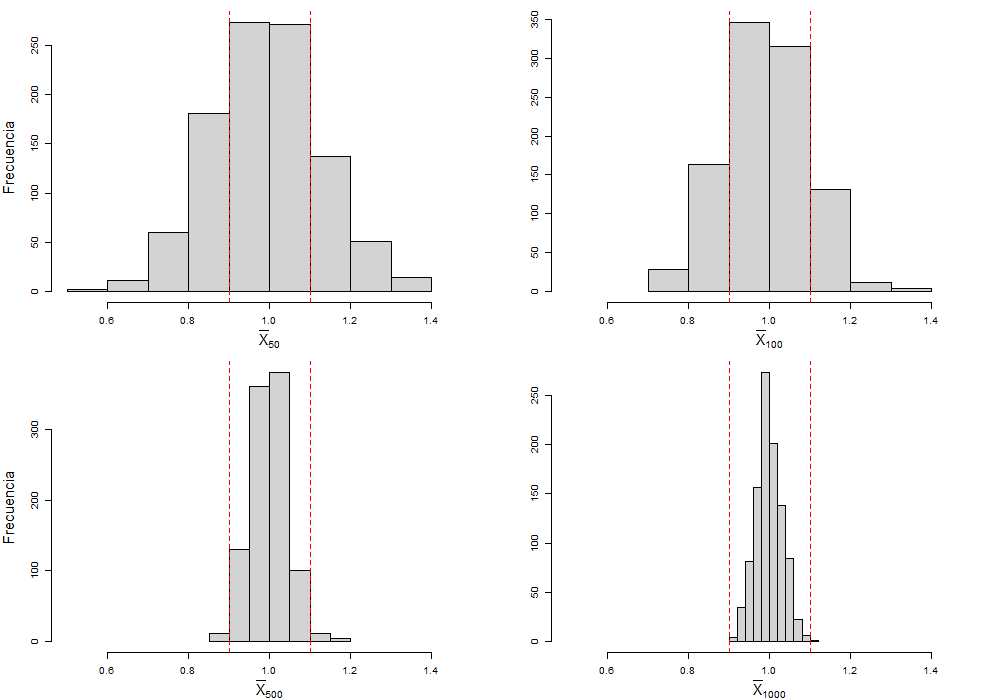
\includegraphics[scale=0.3]{slides1/img/Fig1.png}
    \vspace{-0.1cm}
\caption{Distribución de $\overline{X}_n$ para distintos tamaños de muestra}
\end{figure}
\end{frame}





\begin{frame}{\color{rosee}Demostración de la ley de los grandes n\'umeros para $X_i\stackrel{iid}{\sim}$}\small

  \begin{proof}
    La demostraci\'on general (la que no asume nada sobre Var$(X)$ est\'a fuera del alcanza del curso. Podemos
    probar f\'acilmente que el resultado vale si asumimos que $Var(X)$ es finita. Por Tchebychev, para cualquier $\varepsilon > 0$ vale que 
    \[P\left( \vert \overline{X}_{n}-E(X) \vert \geq
      \varepsilon\right)\leq \frac{Var(\overline{X}_{n})}{\varepsilon^{2}} = \frac{Var(X)}{n} 
    \frac{1}{\varepsilon^{2}}
    \underset{n\to\infty}{\longrightarrow} 0\,.\]
  \end{proof}
  
  \vspace{6pt}
  Usamos que $X_i \stackrel{iid}{\sim}$, lo que nos dice que $E(\overline{X}_n)=E(X)$ y $Var(\overline{X}_n)=Var(X)/n$. ¿En qué parte usamos cada uno de los supuestos?
\end{frame}

\begin{frame}{\color{rosee}LGN para $g(X_i)\stackrel{iid}{\sim}$}\small
  
    Sean $X_{1},\dots,X_{n}\stackrel{iid}{\sim} X$ y $g$ una función continua; entonces vale que $g(X_i)$ \textbf{son variables independientes y son idénticamente distribuidas}. Por lo tanto, para todo $\varepsilon>0$ 
    \begin{equation*}
      P\left( \Big| \frac{1}{n}\sum_{i=1}^ng(X_i)-E(g(X)) \Big| \geq \varepsilon\right)
      \underset{n\to\infty}{\longrightarrow} 0. 
    \end{equation*}
  
\bigskip
\begin{itemize}
    \item %Como quizá habrás notado, este resultado se corresponde con definir $Y_i = g(X_i)$ para $i=1,\dots,n$ y $E(X) = E(Y) = E(g(X))$ y aplicar la LGN para $\overline{Y}_n=\frac{1}{n}\sum_{i=1}^nY_i = \frac{1}{n}\sum_{i=1}^ng(X_i)$. 
    Por ejemplo:\medskip
    \begin{itemize}
   \item Si llamamos $Y_i=g(X_i)=X_i^2$; luego:  \[ \dfrac{1}{n}\displaystyle\sum_{i=1}^{n} X_i^2 = \overline{Y}_n \overset{p}{\to} E(Y) = E(X^2)\]
        \item Si llamamos $Y_i=g(X_i)=\ln(X_i)$; luego: \[\dfrac{1}{n}\displaystyle\sum_{i=1}^{n} \ln(X_i) = \overline{Y}_n \overset{p}{\to} E(Y) = E(\ln(X))\]
    \end{itemize}
    
\end{itemize}

\end{frame}

\begin{frame}{\color{rosee}Algunos ejercicios sobre la LGN para $g(X_i)\stackrel{iid}{\sim}$}\small
%    Es importante que noten que si:
    
%    \begin{itemize}
%     \item $g$ es una función continua, si $X_i=g(Y_i)$ entonces vale que $\dfrac{1}{n}\displaystyle\sum_{i=1}^{n} g(Y_i) \overset{p}{\to} E(g(Y))$
%        \item $X_i=Y_i^2$ entonces vale que $\dfrac{1}{n}\displaystyle\sum_{i=1}^{n} Y_i^2 \overset{p}{\to} E(Y^2)$
%        \item $X_i=\ln(W_i)$ entonces vale que $\dfrac{1}{n}\displaystyle\sum_{i=1}^{n} \ln(W_i) \overset{p}{\to} E(\ln(W))$
%    \end{itemize}
    
    \underline{Ejercicios}
    
    \begin{enumerate}
       \item \noindent Si $X_i\sim_{iid}$, $E(X)=5$ y $Var(X)=144$ calcule $\theta$ si $\dfrac{1}{n}\displaystyle\sum_{i=1}^{n} X_i^2 \overset{p}{\to} \theta$
        
     %   \item \noindent Si $R_i\sim_{iid}$, $E(R)=3$, $Var(R)=16$, diga $\alpha$ / $\dfrac{1}{n}\displaystyle\sum_{i=1}^{n} R_i^{\alpha} \overset{p}{\to} 25$
        
        \item \noindent Si $X_i\sim_{iid}$, $E(X)=1$ y $E(\ln(X))=-1$ calculá $\theta$ si \[\ln\left[\left(\displaystyle\prod_{i=1}^{n} X_i\right)^{\frac{1}{n}}\right] \overset{p}{\to} \theta\]
        
        
        \end{enumerate}
    
\end{frame}

%\section{Teorema Central del L\'imite}

\begin{frame}{\color{rosee}Teorema Central del L\'imite para $X_i\stackrel{iid}{\sim}$} \small
  
 % Recordemos lo que hab\'iamos visto en las simulaciones con R (\S~16):
  %\begin{quote}
%\small{Si $\{X_{1},\dots,X_{n}\}\stackrel{iid}{\sim} X$ y ``$n$ es grande''; la   distribuci\'on de $\overline{X}_{n}$ se concentra alrededor de $E(X)$ y toma una forma similar a la campana normal, aún cuando ladistribuci\'on de $X$ es muy distinta de la normal. Es importante notar que el tamaño de $n$ necesario para que la distribución de $\overline{X}_n$ tenga forma ``normal'' dependerá de la forma de la distribución de $X$. }
%  \end{quote}

  
  \begin{theorem}[Teorema central de l\'imite]
    Sea $X_{1},\dots,X_{n}\stackrel{iid}{\sim} X$ con $E(X)$ y
    $Var(X)$, para todo $z\in\mathbb{R}$
    
    \begin{equation*}
     P\left(\sqrt{n}\frac{ (\overline{X}_{n}-E(X))}{\sqrt{Var(X)}} 
        \leq z \right) \underset{n\to\infty}{\longrightarrow} P(Z \leq z)
    \end{equation*}

  \end{theorem}
  
    \vspace{12pt}
    
    donde $P(Z\leq z)$ con $Z \sim N(0,1)$. A veces se escribe $\Phi(z) = P(Z\leq z)$.
  
  \medskip  
   Escribimos \[\sqrt{n}\frac{ (\overline{X}_{n}-E(X))}{\sqrt{Var(X)}}\overset{d}{\to} N(0,1)\]
\end{frame}

 \begin{frame}{\color{rosee}Observaciones sobre el TCL para $X_i\stackrel{iid}{\sim}$}
\small
  
  \begin{itemize}
  \item   
    El  TCL implica que, si $X_i\sim_{iid}$, entonces para cualesquiera $z_1, z_2 \in \mathbb{R}$ que cumplen que $z_{1} \leq z_{2}$, vale 
    $$
    P\left(z_{1}\leq \frac{ \sqrt{n}\, (\overline{X}_{n}-E(X))}{\sqrt{Var(X)}} 
        \leq z_{2} \right) \underset{n\to\infty}{\longrightarrow} P(Z \leq z_{2}) - P(Z \leq z_{1})
    $$
  \item  El TCL nos va a permitir (m\'as adelante en la materia)   \textit{cuantificar la incertidumbre} (dar un \textbf{margen de error}) que tenemos sobre nuestra estimaci\'on de $E(X)$ usando la media muestral $\overline{X}_n$.
      \item  El teorema se refiere a la distribuci\'on de $\overline{X}_{n}$,
    \textbf{no} a la de $X_{1}, \dots, X_{n}$.
    \item Si $X_i\sim_{iid} N(\mu,\sigma^2)$, \textbf{no es necesario usar TCL} porque vale que, para cualquier $n$ que: $\overline{X}_n\sim N\left(\mu ,\frac{\sigma^2}{n}\right)$.
    \end{itemize}
  
\end{frame}


\begin{frame}{\color{rosee} Notación correcta sobre el TCL para $X_i\stackrel{iid}{\sim}$}\small
\color{-red!70!} \textbf{Notación correcta:}\color{black}
\begin{itemize}
\item \textbf{Distribución asintótica} (versión estandarizada)
\[\frac{\sqrt{n} \,(\overline{X}_{n}-E(X))}{\sqrt{Var(X)}} \stackrel{D}{\to} N(0,1)\]
    \item \textbf{Distribución aproximada} para \textbf{tama\~nos de muestra grande}  ($n\gg 0$), la distribuci\'on de
    $\overline{X}_{n}$ es \textbf{aproximadamente normal}:
    \begin{itemize}
        \item \textbf{Versión estandarizada:} \[\frac{\sqrt{n} \,(\overline{X}_{n}-E(X))}{\sqrt{Var(X)}} \sim_a N(0,1) \text{ si }n \gg 0\]
    \item \textbf{Versión no estandarizada:}
    \[\overline{X}_{n} \sim_a N\left( E(X), \frac{Var(X)}{n} \right)\text{ si } n \gg 0.\]
    \end{itemize}
    \end{itemize}
 %   El TCL nos va a permitir (m\'as adelante en la materia)   \textit{cuantificar la incertidumbre} que tenemos sobre nuestra estimaci\'on de $E(X)$ usando la media muestral $\overline{X}_n$.
    \end{frame}
    
    
 
\begin{frame}{\color{rosee}TCL para $g(X_i)\stackrel{iid}{\sim}$ y ejercicio}\small
Al igual que con la LGN, también vale que si $g$ es una función continua y definimos $Y_i = g(X_i)$ para $i=1,\dots,n$. Luego se cumple que $g(X_i)\stackrel{iid}{\sim}$ y por lo tanto:

$$\sqrt{n}\left[\dfrac{1}{n}\displaystyle\sum_{i=1}^{n} g(X_i) -E(g(X))\right] = \sqrt{n}\big(\overline{Y}_n -E(Y)\big) \overset{d}{\to} N(0,\underbrace{\text{Var}(Y)}_{\text{Var}(g(X))}).$$
    
%    \begin{itemize}
%         \item  \small{Si $X_i=g(Y_i)$ entonces $\sqrt{n}\big(\dfrac{1}{n}\displaystyle\sum_{i=1}^{n} g(Y_i) -E(g(Y))\big)\overset{d}{\to} N(0,Var(g(Y))$} 
   %     \item $X_i=Y_i^2$ \small{entonces vale que} $\sqrt{n}\left[\dfrac{1}{n}\displaystyle\sum_{i=1}^{n} Y_i^2 -E(Y^2)\right]\overset{d}{\to} N(0,Var(X^2))$
 %       \item $X_i=\ln(W_i)$ \small{entonces vale que} $\sqrt{n}\left[\dfrac{1}{n}\displaystyle\sum_{i=1}^{n} \ln(W_i)-E(\ln(W))\right] \overset{d}{\to} N(0,Var(\ln(W))$
 %   \end{itemize}
    
%    \vspace{4pt}
    
    \underline{Ejercicio}
    
    \begin{enumerate}
       \item \noindent Si $X_i\sim_{iid}$, $E(X)=8$ y $Var(X)=225$, $g(X)=X^2$ y $$\sqrt{n}\left[\dfrac{1}{n}\displaystyle\sum_{i=1}^{n} X_i^2 -\theta \right]\overset{d}{\to} N(0,Var(X^2))$$
       
       ¿cuánto vale $\theta$?
       
        
        
 %       \item \noindent Si $S_i\sim_{iid}U(0,\theta)$, calcule\footnote{Tarea: Calcule $Var(\ln(X))$ con Wolfram Alpha y diga cuánto vale $\beta(1)$.} $\beta(\theta)$ si $\sqrt{n}\left[\dfrac{1}{n}\displaystyle\sum_{i=1}^{n} S_i-\beta(\theta) \right]\overset{d}{\to} N(0,Var(\ln(X))$
        
        \end{enumerate}
\end{frame}

%\begin{frame}{\color{rosee}Teorema Central del L\'imite} \small

 % \begin{alertblock}{Idea}
  %  El TCL nos dice que, una versi\'on debidamente re-escalada de
   % $\overline{X}_{n}$ \textbf{converge en cierto sentido} a una
    %distribuci\'on normal $N(0,1)$. Pensemos por qu\'e es razonable este
    %re-escalamiento. Sabemos que
    %\begin{equation*}
     % E(\overline{X}_{n})=\mu \quad Var(\overline{X}_{n})=\frac{\sigma^{2}}{n}.
%    \end{equation*}
 %   Luego
  %  \begin{equation*}
   %   \frac{\sqrt{n}(\overline{X}_{n}-\mu)}{\sigma} = \frac{\overline{X}_{n}
    %    - E(\overline{X}_{n}) }{SD(\overline{X}_{n})}.
    %\end{equation*}
    %El cambio de escala es consiste en 
  %  \begin{itemize}
   % \item restar la esperanza y 
%    \item dividir por el desv\'io!
 %   \end{itemize}
  %  Si $X_{1},\dots,X_{n} \sim N(\mu,\sigma^2)$, entonces la
   % distribuci\'on
    %$\frac{\sqrt{n}(\overline{X}_{n}-\mu)}{\sigma} %\sim
  %  N(0,1)$ es \textbf{exacta}.
 % \end{alertblock}
%\end{frame}



\begin{frame}{\color{rosee}Teorema Central del L\'imite: comentarios}\small
{\color{rosee}¿Qu\'e tan grande debe ser el tamaño de muestra $n$?}
    % Llamemos $X$ a la distribuci\'on que tienen los datos de nuestra
    % muestra aleatoria.
    \begin{itemize}
    \item Si la distribuci\'on de las $X_i$ \textbf{es sim\'etrica}, es decir, si existe
      alg\'un punto $c$ tal que el histograma o la funci\'on de densidad de
      $X$ es sim\'etrica respecto de $c$, t\'ipicamente con $n>20$ la
      aproximaci\'on normal del TCL es adecuada.
    \item Si la distribuci\'on de las $X_i$ \textbf{no es sim\'etrica}, no hay una
      ``receta'' para decir qué tan grande debe ser $n$ para que la distribución de $\overline{X}_n$ se ``parezca'' a una distribución normal. Mientras m\'as grande sea el $n$, ``mejor''.
      \item Para el caso donde $X_i\sim_{iid} Be(p)$ se suele decir que para que la aproximación de la distribución de $\overline{X}_n$ por una distribución normal sea adecuada, debería ocurrir que $np(1-p)>5.$ Notar que esta regla es una \textbf{heurística} y no tiene sustento teórico alguno.
    \end{itemize}

\end{frame}





\begin{frame}{\color{rosee}Teorema Central del L\'imite} \small

  El gobierno de la Ciudad de Buenos Aires est\'a interesado en estimar
  la proporci\'on personas a favor de la ley de etiquetado frontal que habita la Ciudad. Para ello, se entrevistan a $n=100$ personas elegidas al azar de toda
      la poblaci\'{o}n de Argentina y se les pregunta si est\'{a}n a
      favor o en contra de la ley de etiquetado frontal.

        \medskip
  
  Llamemos $X_i=\begin{cases} 0 & \text{ si la persona $i$-\'esima está en contra de la ley}\\ 
   1 & \text{ si la persona $i$-\'esima está a favor de la ley} \end{cases}$
  
  \medskip

    \begin{itemize}[leftmargin=*]

    \item \textbf{Ejercicio 1:} Si el $40\%$ de las personas en Argentina est\'a en contra,
      \begin{itemize}[leftmargin=*]
          
     \item  ¿cu\'{a}l es \textbf{(aproximadamente)} la probabilidad de que en una muestra aleatoria la
      proporci\'{o}n de personas en una muestra aleatoria a favor de la ley de etiquetado frontal %despenalizaci\'{o}n
      est\'{e} entre $0.58$ y $0.62$?
      \item \textbf{acote }(en este caso, dé un valor mínimo de) la probabilidad mecionada en la consigna anterior utilizando la desigualdad de Tchebychev y compare.
      \item Bonus: \textbf{calcule} la probabilidad usando que $100\overline{X}_{100}\sim Bin(100,0.6)$.
    \end{itemize}
    \item \textbf{Ejercicio 2:} ¿Qu\'e valor debe tener el tamaño de muestra $n$ \textbf{como mínimo para garantizar}
  que la proporci\'on de una muestra aleatoria no difiera de la real en m\'as de $0.01$ con una
  probabilidad mayor o igual que $0.95$?
    \end{itemize}
  
\end{frame}



\begin{frame}{\color{rosee}¿Cuándo es razonable suponer que $X_i\stackrel{iid}{\sim}$?} \small 

  Hasta ahora nuestra gran hip\'otesis es que construimos el estimador $\overline{X}_n$ en base a una 
  \textbf{muestra aleatoria} $\{X_1,\dots,X_n\}$ (\textbf{independiencia} +
  \textbf{distribuciones idénticas}). ¿Cuándo es razonable, al menos  aproximadamente, este supuesto?\medskip
  \begin{itemize}
  \item Ej. de etiquetado frontal: Si elegimos a los entrevistados sacando bolillas de un bolillero sin
    reposici\'on y además suponemos que todos responden: s\'i, aproximadamente, porque la poblaci\'on de
    Argentina es grande.\medskip
  \item Si $X_{1},\dots, X_{n}$ son los retornos de un activo financiero en $n$ d\'ias consecutivos de trading: el supuesto iid es poco plausible.
  \begin{itemize}
      \item Lo que ocurra con el retorno en el período $t$ probablemente condicione la distribución del retorno en el/los período/s siguiente/s:
      $$P(X_{t+1}<x) \neq P(X_{t+1}<x|X_{t}=c).$$
      \item No id: La varianza cambia a lo largo del tiempo. \medskip
  \end{itemize}
  \item Si $X_{1},\dots, X_{n}$ son ventas mensuales de cerveza en $n$ meses consecutivos: no, no van a ser independientes, ¡dependencia temporal y estacionalidad!
  \end{itemize}
\end{frame}



%\begin{frame}{\color{rosee}Teorema Central del L\'imite} \small
%  
%  \begin{example}
%    La fracci\'on de soja que es considerada de buena calidad en las
%    silobolsas de un gran productor agropecuario es una variable
%    aleatoria $X$ con densidad $f_{X}(x)=(4/3)(1-x^3)$ si $0<x<1$ y
%    $f_X(x)=0$ en otro caso. Supongamos que del total de silobolsas
%    del productor se eligen $200$ al azar de manera independiente.
%    \begin{enumerate}
%    \item Indicar la distribuci\'on de la variable aleatoria
%      $N=$ ``n\'umero de silobolsas en la muestra con una
%      fracci\'on de soja de buena calidad mayor al $50\%$''.
%    \item Usando el TCL, aproximar la probabilidad de que a lo sumo
%      $30\%$ de las silobolsas de la muestra tengan una fracci\'on de
%      soja de buena calidad mayor al $50\%$.
%    \item Usando el TCL, aproximar la probabilidad de que la fracci\'on
%      promedio de soja de buena calidad en la muestra sea mayor al
%      $39\%$.
%    \end{enumerate}
%  \end{example}
%\end{frame}

\begin{frame}{\color{rosee}Animaciones} 

Para visualizar LGN y TCL

\url{https://onlinestatbook.com/stat_sim/sampling_dist/index.html}

\vspace{18pt}

Otras páginas

\url{https://seeing-theory.brown.edu/}

 \url{https://pianophase.shinyapps.io/distribuciones-muestrales/}
\end{frame}

% \begin{frame}{\color{rosee}Teorema Central del L\'imite}
%   \small
%   \begin{example}
%     \begin{itemize}
%     \item
%       Sea $X_{i}=1$ si la persona $i$ en la muestra est\'{a} en contra de la
%       despenalizaci\'{o}n, y $X_{i}=0$ en caso contrario.
%       
%     \item Sea
%       \[
%       \overline{X}_{200}=\frac{1}{200}\sum_{i=1}^{200}X_{i}%
%       \]
%       
%     \item $\overline{X}_{200}$ es la proporci\'{o}n de personas en contra de la
%       despenalizaci\'{o}n en tu encuesta.
%       
%     \item Como la premisa dice que el 40\% de la poblaci\'{o}n est\'{a} en contra
%       de la despenalizaci\'{o}n, entonces sabemos que $X_{i}\sim Ber\left(
%         0.4\right).$
%       
%     \item Adem\'{a}s, como la poblaci\'{o}n de Argentina es muy grande, podemos
%       asumir que $X_{1},...,X_{200}$ son independientes.
%     \end{itemize}%
%   \end{example}
% \end{frame}
% 
% \begin{frame}{\color{rosee}Teorema Central del L\'imite}
%   \small
%   \begin{example}
%     
%   \end{example}
% \end{frame}

\end{document}
\begin{frame}[noframenumbering]{}
\begin{center}
\Large    

    Apéndice
    (las slides a partir de aquí son optativas)
    \end{center}
\end{frame}

\begin{frame}[noframenumbering]{\textcolor{gray}{Demostraci\'on de la desigualdad de Markov \S3}} \small
Lo probamos para variables aleatorias discretas y utilizando el resultado particular:
    \begin{equation*}
      A \equiv \left\lbrace x:  x  < \varepsilon \right\rbrace.      
    \end{equation*}
Llamemos $I_{A}(x)$ a la función indicadora del conjunto $A$, es decir que $I_{A}(x)=1$ si $x\in A$ e $I_{A}(x)=0$ en otro caso, entonces:
    \begin{align*}
      E( X )=\sum\limits_{x} x p_{X}(x)
      &=\sum\limits_{x} x p_{X}(x) I_{A}(x)+ 
        \sum\limits_{x} x p_{X}(x) I_{A^{c}}(x)\\
      & \geq \sum\limits_{x} x p_{X}(x) I_{A^{c}}(x) \\
      & \geq \varepsilon \sum\limits_{x}  p_{X}(x) I_{A^{c}}(x) \\
      & \geq \varepsilon P\left( X \in A^{c}\right) = \varepsilon
        P\left( X \geq \varepsilon\right)
    \end{align*}
Para demostrar el caso general considerá $A \equiv \left\lbrace x:  g(x)  < \varepsilon \right\rbrace$.
    \end{frame}


\begin{frame}[fragile,noframenumbering]{\color{rosee}Ley de los grandes n\'umeros \S14}\small
  \begin{lstlisting}
grilla_n     <- c(50,100,500,1000)
medias.estim <- matrix(0, ncol = 4, nrow = 1000)
for (i in 1:4){
  muestras <- replicate(1000, 
                        rpois(n = grilla_n[i], 
                        lambda = 1))
  medias.estim[,i] <- colMeans(muestras)
}
par(mfrow = c(2,2), mar = c(4,4,1,1))
hist(medias.estim[,1], ylab = 'Frecuencia'
     xlab = expression(bar(X)[n=50]))
hist(medias.estim[,2], ylab = ''
     xlab = expression(bar(X)[n=100])))
hist(medias.estim[,3], ylab = 'Frecuencia'
     xlab = expression(bar(X)[n=500]))
hist(medias.estim[,4], ylab = ''
     xlab = expression(bar(X)[n=1000]))
  \end{lstlisting}
  
  Simulamos 1000 realizaciones de $\overline{X}_{n}$ cuando $X\sim \text{Poiss}(\lambda=1)$ considerando diferentes valores de $n\in \{50,100,500,1000\}$ (resumen en la gráfica de \S14). 
\end{frame}

\begin{frame}[noframenumbering]{\color{rosee}Boxplots}
    \begin{figure}
\centering
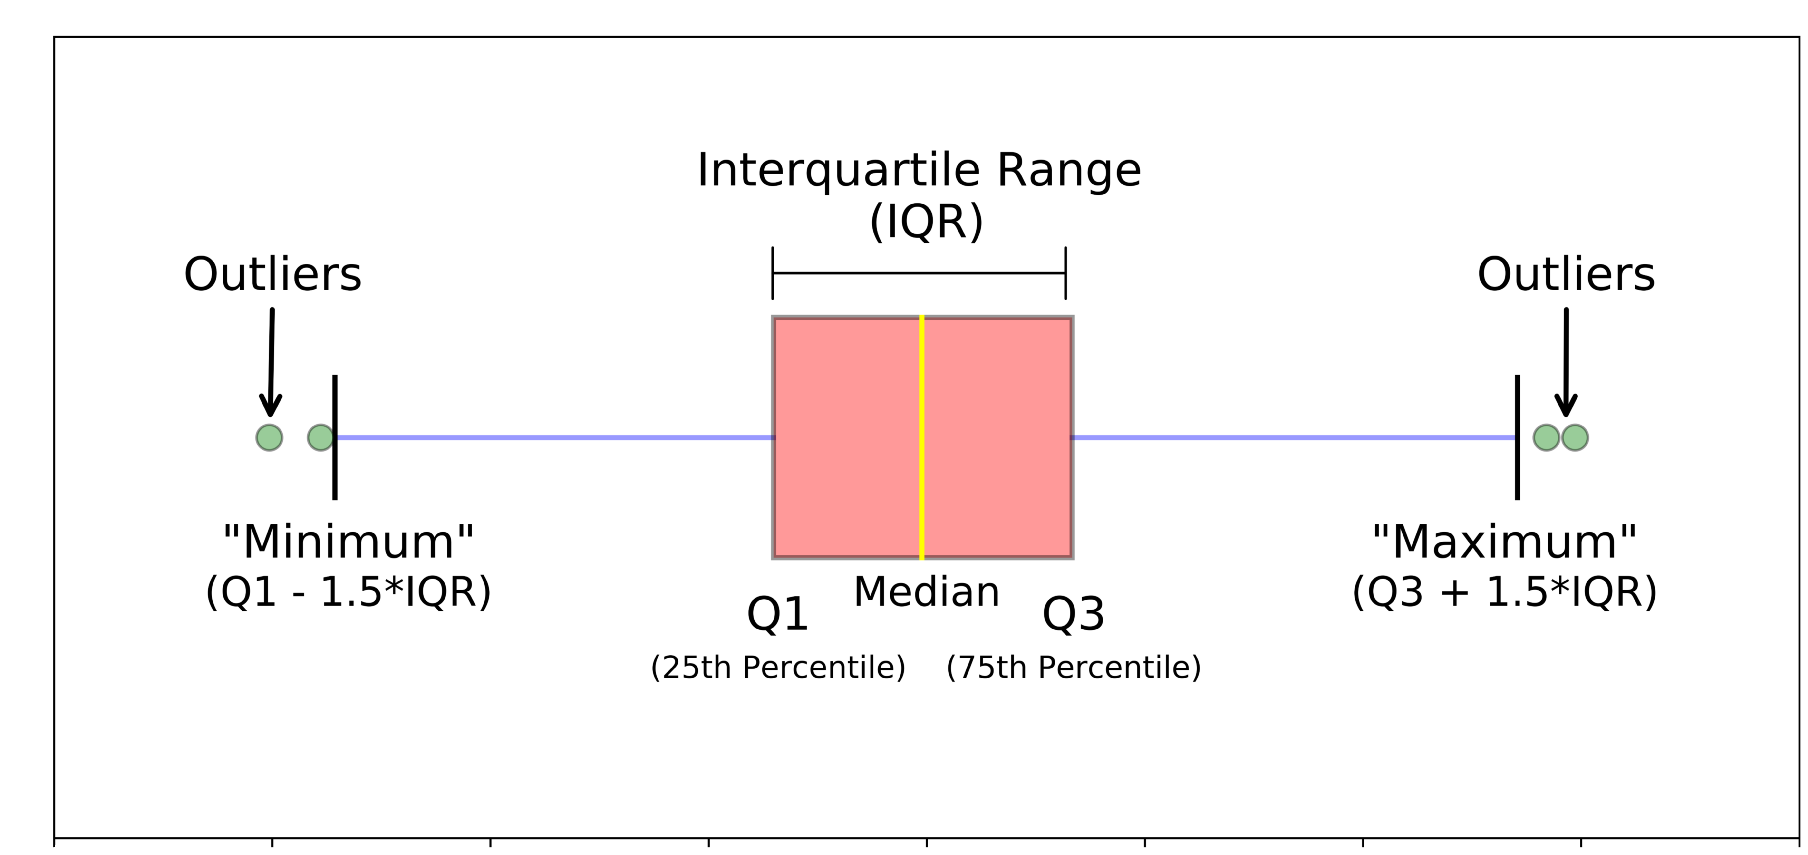
\includegraphics[scale=.33]{slides1/img/boxplot_def.png} 
\caption{Las gráficas de cajas o boxplots  nos permiten visualizar la distribución empírica de los datos concentrándonos en los cuartiles.} 
\end{figure}
\begin{itemize}
    \item Volvamos a visualizar en 4 gráficos de caja las distribuciones empíricas (las distintas realizaciones) de $\overline{X_n}$ para los tamaños de muestra que consideramos en la simulación con \texttt{R}.
\end{itemize}
\end{frame}


\begin{frame}[noframenumbering]{\color{rosee} Distribución empírica de $\overline{X}_n$ con boxplots, $X_i \stackrel{iid}{\sim} Poi(1)$.}
\begin{figure}
    \centering
    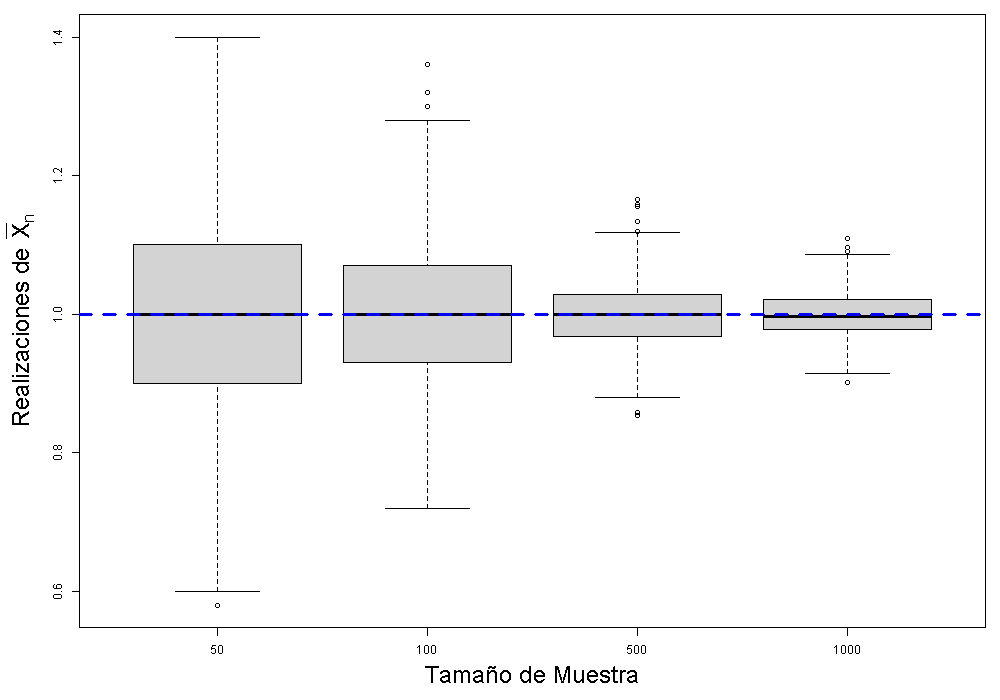
\includegraphics[scale=0.3]{slides1/img/Fig2.png}
    \vspace{-0.2cm}
\caption{Distribución empírica de $\overline{X}_n$ (en azul el verdadero valor de $\lambda = 1$).}
\end{figure}
\end{frame}

\begin{frame}[fragile,noframenumbering]{\color{rosee}Teorema Central del L\'imite \S24}\small
  \begin{lstlisting}
    n_muestra <- 50
    n_rep <- 1000
    parametro <- 0.5  # asimetrica 0.95 o 0.05
    esperanza <- parametro
    desvio <- sqrt(parametro*(1-parametro))
    escalar <- FALSE
    muestras <- replicate(n=n_rep,
                          rbinom(n=n_muestra, size=1, 
                                 prob=parametro))
    medias <- colMeans(muestras)
    par(mfrow=c(1, 2))
    hist(medias, col="steelblue", angle=45, density=20,
         freq=FALSE, main="Histograma de medias",
         xlab="Medias", xlim=c(0, 1))
    hist(sqrt(n_muestra)*(medias-esperanza)/desvio,
         col="steelblue", angle=45, density=20,
         freq=FALSE, main="Histograma de medias",
         xlab="Medias")#, xlim=c(0, 1))
    curve(dnorm(x), add=TRUE, col="darkorange", 
          lwd=3, lty=2)
  \end{lstlisting}
\end{frame}


\end{document}